\documentclass[11pt]{article}

\usepackage[margin=1in]{geometry}
\usepackage{amsmath}
\usepackage{amssymb}
\usepackage{booktabs}
\usepackage{graphicx}
\usepackage{hyperref}

\title{AI in Space: A First Autonomous Rendezvous Simulation}
\author{Fabio Facin}
\date{May 2026}

\begin{document}

\maketitle

\begin{abstract}
This paper defines the starting point for a long-term research project on autonomous spacecraft decision-making.
The project combines orbital mechanics, numerical simulation, artificial intelligence, and later extensions into nuclear-electric propulsion, spacecraft power management, and relativistic navigation corrections.
The first experiment is intentionally simple: a chaser spacecraft in low Earth orbit must choose thrust actions that reduce its relative distance to a target spacecraft while limiting relative velocity and fuel use.
We introduce a first custom decision formula, the Rendezvous Intent Functional, and test it in both Python and C++ implementations.
\end{abstract}

\section{Motivation}

The goal of this project is to build an extensible simulation environment where spacecraft autonomy can be tested under increasingly realistic physical constraints.
Rather than beginning with a fully trained neural network, we begin with a transparent decision rule that can be inspected, modified, and compared against future learning-based agents.

This direction is useful because autonomous spacecraft will need to make decisions when direct human control is delayed, unavailable, or too slow.
Examples include satellite inspection, debris avoidance, lunar logistics, asteroid missions, deep-space navigation, and high-power electric propulsion missions.
The long-term version of this project will let an agent reason about orbit, fuel, power, heat, sensor uncertainty, communication delay, radiation, and mission risk.

\section{First Scenario}

The first scenario is planar autonomous rendezvous.
There are two spacecraft:

\begin{itemize}
    \item a target spacecraft in a circular orbit at altitude \(500~\mathrm{km}\),
    \item a chaser spacecraft in a nearby circular orbit at altitude \(485~\mathrm{km}\), initially behind the target by \(0.045~\mathrm{rad}\).
\end{itemize}

The Earth gravitational parameter is
\[
    \mu_E = 398600.4418~\mathrm{km^3/s^2},
\]
and the Earth radius used in the simulation is
\[
    R_E = 6378.137~\mathrm{km}.
\]

The target and chaser orbital radii are therefore
\[
    r_T = R_E + 500 = 6878.137~\mathrm{km},
    \qquad
    r_C = R_E + 485 = 6863.137~\mathrm{km}.
\]

For a circular orbit, the speed is
\[
    v = \sqrt{\frac{\mu_E}{r}}.
\]
This gives
\[
    v_T = 7.6126~\mathrm{km/s},
    \qquad
    v_C = 7.6209~\mathrm{km/s}.
\]

\section{Dynamics Model}

The first model uses two-body orbital dynamics with an optional thrust acceleration:
\[
    \ddot{\mathbf r}
    =
    -\mu_E \frac{\mathbf r}{\|\mathbf r\|^3}
    +
    \mathbf a_T.
\]

Here \(\mathbf r \in \mathbb R^2\) is the spacecraft position vector, and \(\mathbf a_T\) is the commanded thrust acceleration.
The target spacecraft is propagated with \(\mathbf a_T = \mathbf 0\).
The chaser may choose one of five discrete actions:

\[
    \mathcal A =
    \{\text{coast}, \text{prograde}, \text{retrograde}, \text{radial-out}, \text{radial-in}\}.
\]

The maximum thrust acceleration in this first run is
\[
    a_{\max} = 2.0 \times 10^{-5}~\mathrm{km/s^2}
    =
    0.02~\mathrm{m/s^2}.
\]

The numerical propagator is fourth-order Runge--Kutta with timestep
\[
    \Delta t = 10~\mathrm{s}.
\]

\section{The First Custom Formula}

At each decision time \(t_k\), the agent evaluates every candidate action \(a \in \mathcal A\).
Each candidate action is held constant over a lookahead horizon
\[
    H = 900~\mathrm{s}.
\]

Let the relative position and velocity after the lookahead be
\[
    \boldsymbol\rho_H(a) = \mathbf r_C(t_k + H; a) - \mathbf r_T(t_k + H),
\]
\[
    \boldsymbol\nu_H(a) = \mathbf v_C(t_k + H; a) - \mathbf v_T(t_k + H).
\]

Let the closest predicted distance during the lookahead be
\[
    d_{\min}(a)
    =
    \min_{\tau \in [0,H]}
    \left\|
    \mathbf r_C(t_k+\tau; a) - \mathbf r_T(t_k+\tau)
    \right\|.
\]

The first personalized decision formula for this project is the \textbf{Rendezvous Intent Functional}:

\[
\boxed{
    \mathcal J_{\mathrm{RIF}}(a;t_k)
    =
    \|\boldsymbol\rho_H(a)\|
    +
    \lambda_v \|\boldsymbol\nu_H(a)\|
    +
    \lambda_c d_{\min}(a)
    +
    \lambda_f \Delta v_a
}
\]

The selected action is
\[
    a^*(t_k)
    =
    \arg\min_{a \in \mathcal A}
    \mathcal J_{\mathrm{RIF}}(a;t_k).
\]

\subsection{Meaning of Each Term}

The term \(\|\boldsymbol\rho_H(a)\|\) rewards actions that reduce the predicted range to the target after the lookahead horizon.

The term \(\lambda_v \|\boldsymbol\nu_H(a)\|\) penalizes high relative velocity.
This matters because rendezvous is not just about getting close; the chaser must also arrive gently enough to remain controllable.

The term \(\lambda_c d_{\min}(a)\) is a first-pass closeness-seeking term.
In this initial no-debris scenario, smaller closest approach is useful, so this term helps the planner prefer actions that create an actual rendezvous opportunity.
In future debris or docking scenarios, this term should be replaced or combined with a safety barrier that penalizes being too close at unsafe speeds.

The term \(\lambda_f \Delta v_a\) penalizes fuel use.
For a constant burn over the lookahead horizon,
\[
    \Delta v_a =
    \begin{cases}
    0, & a = \text{coast}, \\
    a_{\max}H, & a \neq \text{coast}.
    \end{cases}
\]

The current simulation uses the unnormalized implementation
\[
    \mathcal J_{\mathrm{run}}(a;t_k)
    =
    D_H(a)
    +
    900 V_H(a)
    +
    0.2 D_{\min}(a)
    +
    C_f(a),
\]
where \(D_H\) is in kilometers, \(V_H\) is in kilometers per second, and \(C_f\) is a small burn penalty.
This is not meant to be the final objective function.
It is the first testable version: simple enough to understand, but structured enough to evolve.

\section{What We Are Testing}

This first paper tests four basic ideas:

\begin{enumerate}
    \item whether a short-horizon action evaluator can reduce target distance without being explicitly taught a Hohmann transfer,
    \item whether relative velocity can be included in the same formula as position error,
    \item whether the same physics can be implemented consistently in Python and C++,
    \item whether this formula gives us a foundation that can later become a reinforcement learning reward or model predictive control objective.
\end{enumerate}

\section{First Simulation Result}

The first simulation ran for up to \(7200~\mathrm{s}\), with a new decision every \(60~\mathrm{s}\).
The success condition was
\[
    \|\boldsymbol\rho\| \leq 5~\mathrm{km}
    \qquad \text{and} \qquad
    \|\boldsymbol\nu\| \leq 0.020~\mathrm{km/s}.
\]

\begin{table}[h]
\centering
\begin{tabular}{lr}
\toprule
Quantity & Value \\
\midrule
Initial range & \(309.52~\mathrm{km}\) \\
Final range & \(4.89~\mathrm{km}\) \\
Minimum range & \(4.89~\mathrm{km}\) \\
Final relative speed & \(0.0128~\mathrm{km/s}\) \\
Approximate \(\Delta v\) used & \(80.6~\mathrm{m/s}\) \\
Simulated time to success & \(90.2~\mathrm{min}\) \\
\bottomrule
\end{tabular}
\caption{First autonomous rendezvous result using the Rendezvous Intent Functional.}
\end{table}

\begin{figure}[h]
\centering
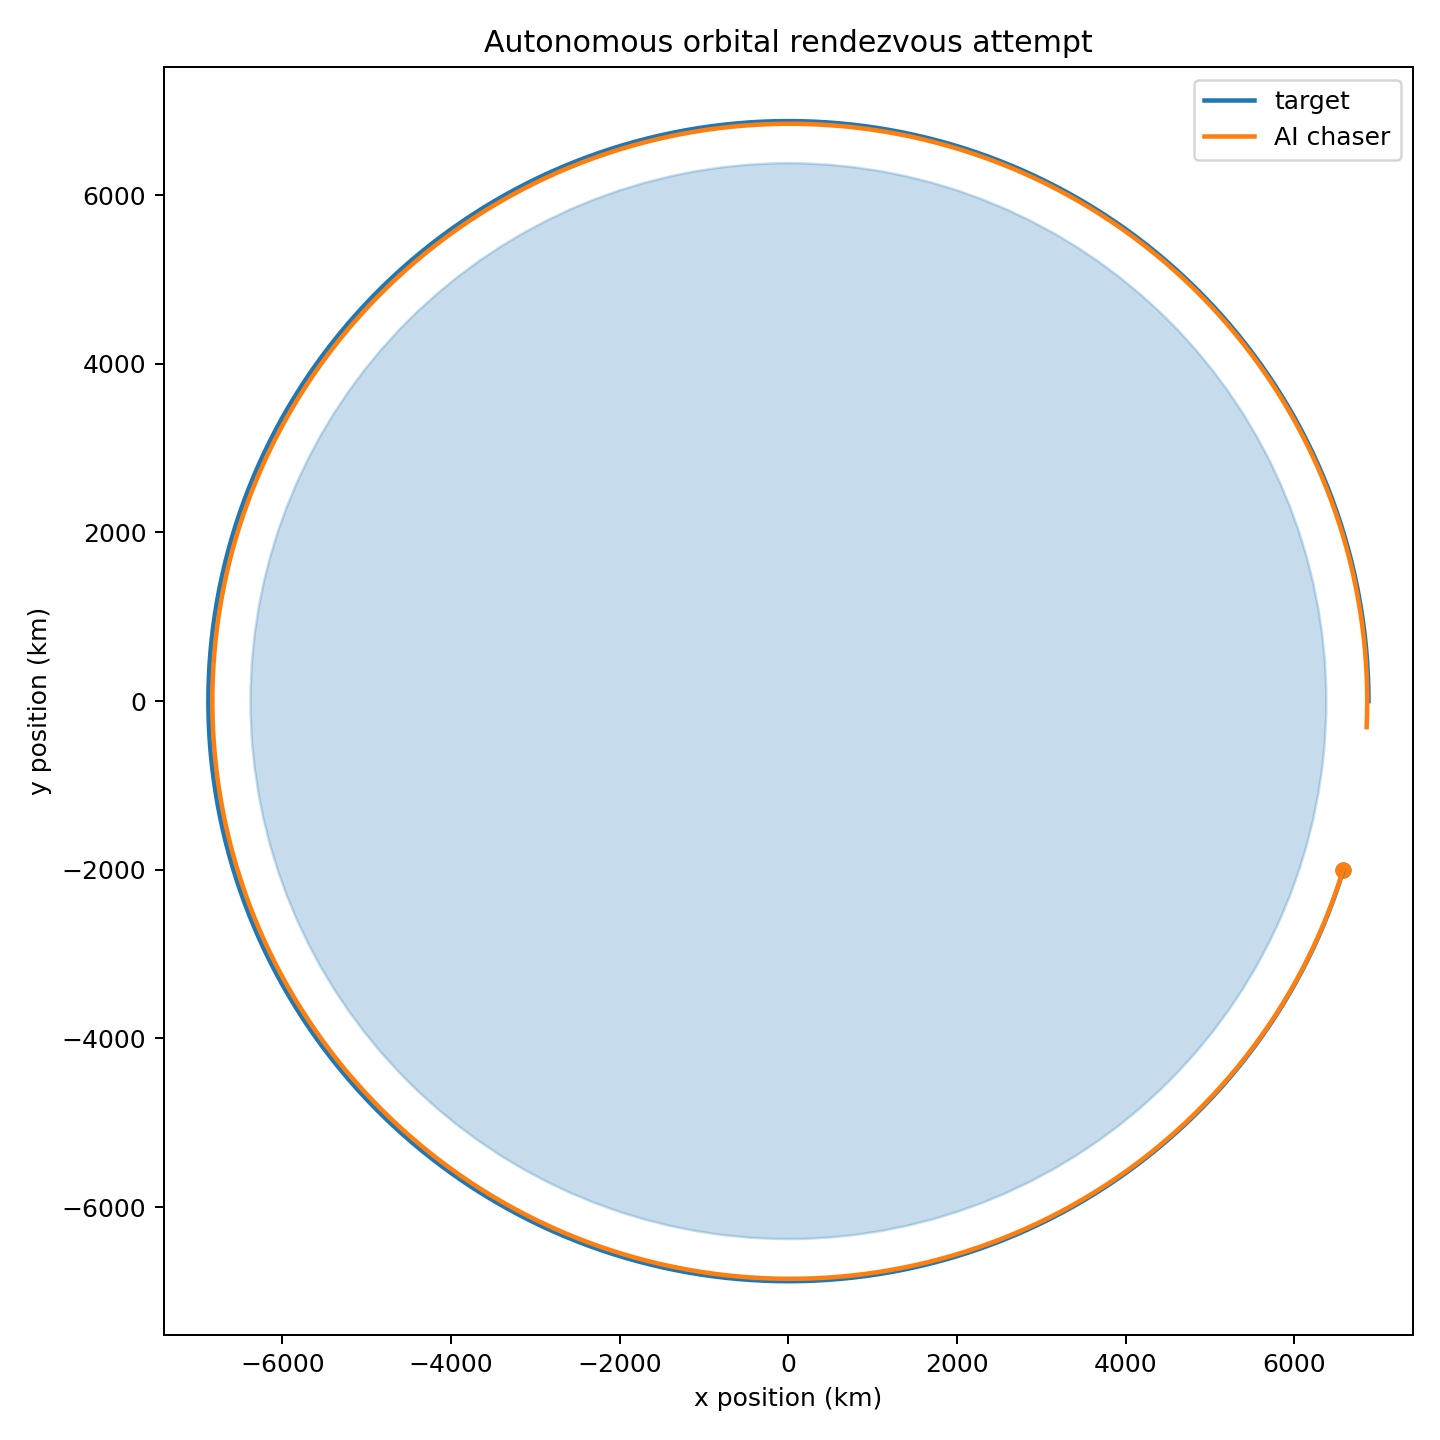
\includegraphics[width=0.78\linewidth]{../simulations/first_rendezvous/trajectory.png}
\caption{Target and chaser trajectories for the first autonomous rendezvous attempt.}
\end{figure}

\begin{figure}[h]
\centering
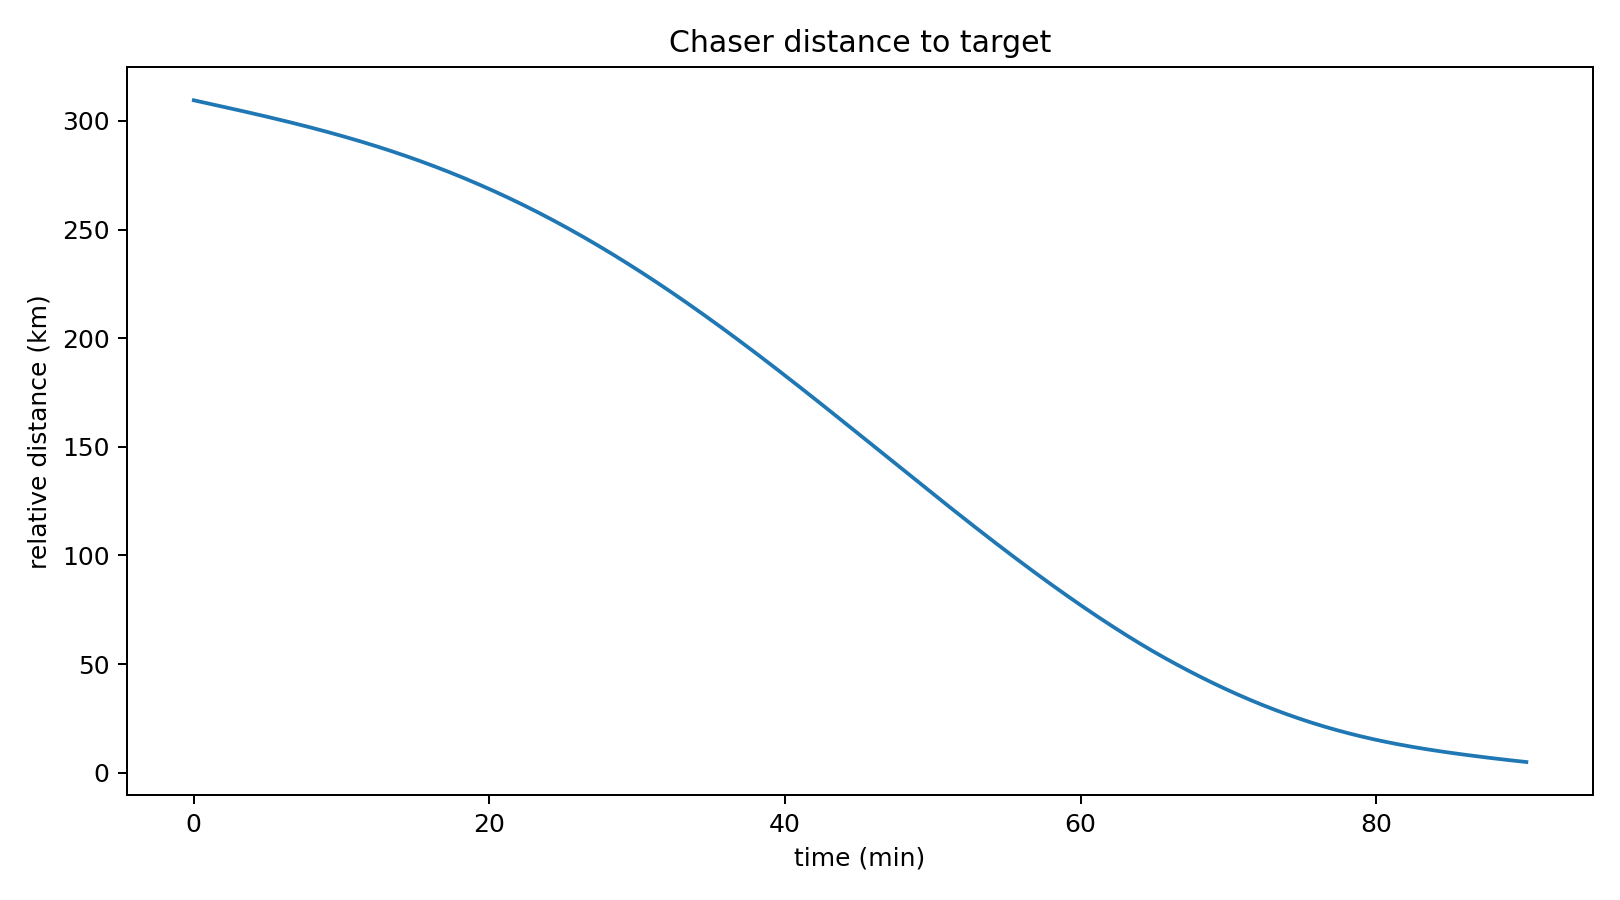
\includegraphics[width=0.78\linewidth]{../simulations/first_rendezvous/distance.png}
\caption{Relative distance between the chaser and target over time.}
\end{figure}

\section{Discussion}

The result is promising because a very simple action evaluator was able to reduce range from roughly \(310~\mathrm{km}\) to under \(5~\mathrm{km}\) while satisfying the relative-speed constraint.
This does not mean the agent is intelligent in the final sense.
It means the project now has a working decision loop:

\[
    \text{state}
    \rightarrow
    \text{candidate actions}
    \rightarrow
    \text{physics rollout}
    \rightarrow
    \text{score}
    \rightarrow
    \text{chosen action}.
\]

That loop is exactly what we need before introducing reinforcement learning.
A neural policy can eventually learn to approximate or improve this decision process, while the transparent formula remains useful as a baseline.

\section{Next Steps}

The next version should introduce a normalized objective:
\[
    \tilde{\mathcal J}(a;t_k)
    =
    w_r \frac{\|\boldsymbol\rho_H(a)\|}{r_{\mathrm{ref}}}
    +
    w_v \frac{\|\boldsymbol\nu_H(a)\|}{v_{\mathrm{ref}}}
    +
    w_f \frac{\Delta v_a}{\Delta v_{\mathrm{ref}}}
    +
    w_s B(a),
\]
where \(B(a)\) is a safety barrier term.
For example, a future debris-aware version could use
\[
    B(a)
    =
    \sum_i
    \frac{1}{\max(d_i(a)-d_{\mathrm{safe}}, \epsilon)^2},
\]
where \(d_i(a)\) is the predicted distance to object \(i\), \(d_{\mathrm{safe}}\) is the required safety distance, and \(\epsilon\) prevents division by zero.

After this, the project should add:

\begin{itemize}
    \item debris avoidance,
    \item sensor noise,
    \item continuous thrust,
    \item low-thrust electric propulsion,
    \item battery and reactor power constraints,
    \item thermal/radiator limits,
    \item reinforcement learning agents trained against the same environment.
\end{itemize}

\section{Conclusion}

This first paper defines the foundation of the AI in Space project.
The first simulation is deliberately small, but it already combines orbital mechanics, numerical integration, autonomous action selection, and measurable success criteria.
The Rendezvous Intent Functional is the first custom formula in the project.
It is not final; it is a testable starting point that can evolve into safer, more physically complete, and more intelligent decision-making methods.

\section{Long-Term Aim: The Spacecraft Autonomy Functional}

The long-term aim of this project is to move from a rendezvous-only score to a general mission decision formula.
The formula below is not something this first simulation has proven.
Instead, it is the direction we are aiming toward: a single objective that lets an autonomous spacecraft balance mission progress, fuel, safety, power, heat, uncertainty, and timing.

We call this target formula the \textbf{Spacecraft Autonomy Functional}:

\[
\boxed{
\begin{aligned}
    \mathcal J_{\mathrm{SAF}}(a;t)
    =
    &\,w_m \Phi_{\mathrm{mission}}(x_{t+H})
    + w_r \frac{\|\boldsymbol\rho_H(a)\|}{r_{\mathrm{ref}}}
    + w_v \frac{\|\boldsymbol\nu_H(a)\|}{v_{\mathrm{ref}}}
    + w_f \frac{\Delta v_a}{\Delta v_{\mathrm{ref}}}
    \\
    &+ w_p \frac{P_{\mathrm{req}}(a)}{P_{\mathrm{avail}}}
    + w_q \frac{Q_{\mathrm{thermal}}(a)}{Q_{\mathrm{limit}}}
    + w_s \mathcal B_{\mathrm{safety}}(a)
    + w_u \mathrm{tr}\!\left(\Sigma_{t+H}(a)\right)
    + w_\tau \left|\frac{\Delta \tau_{\mathrm{rel}}(a)}{\tau_{\mathrm{ref}}}\right|.
\end{aligned}
}
\]

The autonomous spacecraft should choose
\[
    a^*(t)
    =
    \arg\min_{a \in \mathcal A}
    \mathcal J_{\mathrm{SAF}}(a;t).
\]

Each term represents a future research layer:

\begin{itemize}
    \item \(\Phi_{\mathrm{mission}}\): mission progress, such as inspection completion, docking readiness, transfer accuracy, or cargo delivery.
    \item \(\|\boldsymbol\rho_H\|/r_{\mathrm{ref}}\): normalized future position error.
    \item \(\|\boldsymbol\nu_H\|/v_{\mathrm{ref}}\): normalized future relative velocity error.
    \item \(\Delta v_a/\Delta v_{\mathrm{ref}}\): normalized propellant or maneuver cost.
    \item \(P_{\mathrm{req}}/P_{\mathrm{avail}}\): power demand relative to available spacecraft power.
    \item \(Q_{\mathrm{thermal}}/Q_{\mathrm{limit}}\): thermal load relative to radiator or component limits.
    \item \(\mathcal B_{\mathrm{safety}}\): collision, keep-out-zone, radiation, or hardware-limit barriers.
    \item \(\mathrm{tr}(\Sigma_{t+H})\): predicted navigation uncertainty, where \(\Sigma\) is the state-estimation covariance.
    \item \(\Delta \tau_{\mathrm{rel}}/\tau_{\mathrm{ref}}\): relativistic timing correction, useful later for precision navigation and clock-sensitive missions.
\end{itemize}

This formula gives the project a north star.
The first Rendezvous Intent Functional is a small subset of it.
As the simulator grows, each term can become a separate experiment: first orbital motion, then collision safety, then uncertainty, then power and thermal constraints, then nuclear-electric propulsion, and eventually relativistic navigation corrections.

\end{document}
